\documentclass[11pt]{article}
\usepackage[margin=1in]{geometry}
\usepackage{amsmath,amssymb}
\usepackage{graphicx}
\usepackage{hyperref}
\usepackage{enumitem}
\usepackage{xcolor}
\usepackage{titlesec}
\usepackage{authblk}

\hypersetup{
    colorlinks=true,
    linkcolor=blue,
    urlcolor=blue,
    citecolor=blue
}

\titleformat{\section}{\large\bfseries}{\thesection.}{0.5em}{}
\titleformat{\subsection}{\normalsize\bfseries}{\thesubsection}{0.5em}{}

\graphicspath{{figs/}}

\title{\textbf{E\textsuperscript{2}-JEPA: From Free Energy to Automatic Hierarchy}}

\author{Jiaqi Wang}
\affil{Eindhoven University of Technology \\ \texttt{ghazziwang2000@outlook.com}}

\date{}

\begin{document}

\maketitle

\begin{abstract}
Long-horizon control requires hierarchy, and hierarchy requires knowing which latent dimensions stay valid for long horizons. We measure this directly---the relaxation time $\tau$ of each latent dimension---and find a universal failure: across five self-trained JEPA regimes and an independent published world model, the sorted $\tau$ spectrum never shows a gap larger than $1.03$, so no hierarchy boundary can be placed anywhere. The diagnosis is causal: the underlying dynamics \emph{do} contain multi-scale structure, but a scalar-temperature entropy regularizer cannot organize the coordinates, because compressed representations leave no room for organization while overcomplete ones are homogenized by dense normalization. Entropy is moreover an existence precondition: collapsed representations exhibit pseudo-slow $\tau$ with zero information, so any fix must live inside a free-energy objective and act differentially across scales. We therefore constructed the first-principles candidate under these constraints---a \textbf{temperature vector}, $F = U - \sum_k T_k S_k$ over latent bands---and tested it under preregistered acceptance criteria. It fails informatively: every redistribution metric moves in the intended direction, but the inter-band ratio reaches only $1.11$ against a required $1.5$, because temperature governs the \emph{survival} of information, not its \emph{placement}, while the prediction energy can only remove content, never place it. Organizing latents by time scale therefore remains genuinely open; this proposal contributes the referee (the $\tau$ protocol), the discipline (preregistered falsification loops), and the endgame (a subgoal backtest) with which to explore it.
\end{abstract}

\section{Introduction}

Joint-Embedding Predictive Architectures (JEPAs) learn world models by predicting in representation space rather than observation space, avoiding the cost of pixel-level reconstruction while producing compact latents suitable for planning~\cite{lecun2022path,assran2023ijepa}. For long-horizon control, however, prediction alone is not enough: the planner must decide \emph{at which temporal scale each piece of latent information is valid}. When hierarchical world models ignore this and treat upper-level predictions directly as subgoals for the lower level, policy success degrades from $73.3\%$ (oracle subgoals) to $38.7\%$~\cite{hilewm2026}---the interface fails precisely because nothing marks which latents are coarse enough to serve as goals and which are not.

Recent work has begun interrogating the forward-prediction objective itself. PSG-JEPA observes that forward prediction does not enforce reliable identifiability of physical state, and adds proprioceptive grounding as a training-time auxiliary~\cite{psgjepa2026}. Our work addresses the orthogonal deficiency that remains even when latents are identifiable: \emph{temporal unorganization}. We ask: \emph{can the training objective itself organize latent dimensions by their characteristic time scale, so that hierarchy emerges from first principles rather than architectural heuristics?}

\section{A Measurable Notion of Temporal Scale}

We define the granularity of a latent dimension as its characteristic relaxation time $\tau_i$: the duration over which dimension $i$ stays correlated with its own past. This is the physicist's correlation time---the quantity that separates slow from fast modes in statistical mechanics and sets the coarse-graining axis of the renormalization group---lifted from molecular observables to latent coordinates. We estimate $\tau$ with two independent estimators, because each is blind to what the other sees.

\textbf{Estimator A (data side).} For each dimension, integrate its autocorrelation function $C_i(\Delta)$ over lags $\Delta$, truncating at the first non-positive lag (the initial-positive-sequence rule, which prevents noise at large lags from cancelling real signal). This estimator uses trajectories only; no model is involved.

\textbf{Estimator B (model side).} Linearize the learned one-step latent dynamics $f$ at data points to obtain the Jacobian $J = \partial f / \partial z$, and convert each eigenvalue to a time scale via $\tau = -1/\ln|\lambda|$. This estimator uses the model only; no data statistics are involved.

\textbf{Why the metric can be trusted.} Three properties, established in Section~3, carry it. First, the two estimators are independent---one reads data trajectories, the other reads the learned dynamics---so agreement certifies structure and disagreement localizes artifacts. Second, the protocol calibrates against ground truth where one exists: on the external model it recovers exactly the dimension of the physical state (Section~3.2), a number known independently of anything we trained. Third, the metric declares its own failure modes: it is undefined on collapsed representations rather than silently returning pseudo-slow readings (Section~3.4). A measurement that can be calibrated, cross-checked, and made to fail loudly is one whose positives can be believed. A hierarchy boundary, if any, should be placed at the largest multiplicative \emph{gap} in the sorted $\tau$ spectrum; the empirical finding is that this gap does not exist. Section~4 reports the first attempt to create it, and what its failure teaches.

\section{Preliminary Results: The Collapse Is Real, Universal, and Diagnosed}

The measurement phase is complete. All numbers below are measured on PushT teleoperation data with the protocol of Section~2; none are projected.

\subsection{Universal spectral gap collapse}

We trained five regimes---energy-only (no entropy term), JEPA, E$^2$-JEPA, behavior cloning (BC), and flow-matching BC---under identical data. We additionally audited the published LeWM PushT world model~\cite{lewm2026}, which is deployed for model-predictive control, on its own released training set. In every case the sorted $\tau$ spectrum is gapless: the maximum ratio between consecutive values is $\le 1.03$ (Fig.~\ref{fig:collapse}). No training objective, no model scale, and no anti-collapse mechanism produced a natural hierarchy boundary.

\begin{figure}[t]
    \centering
    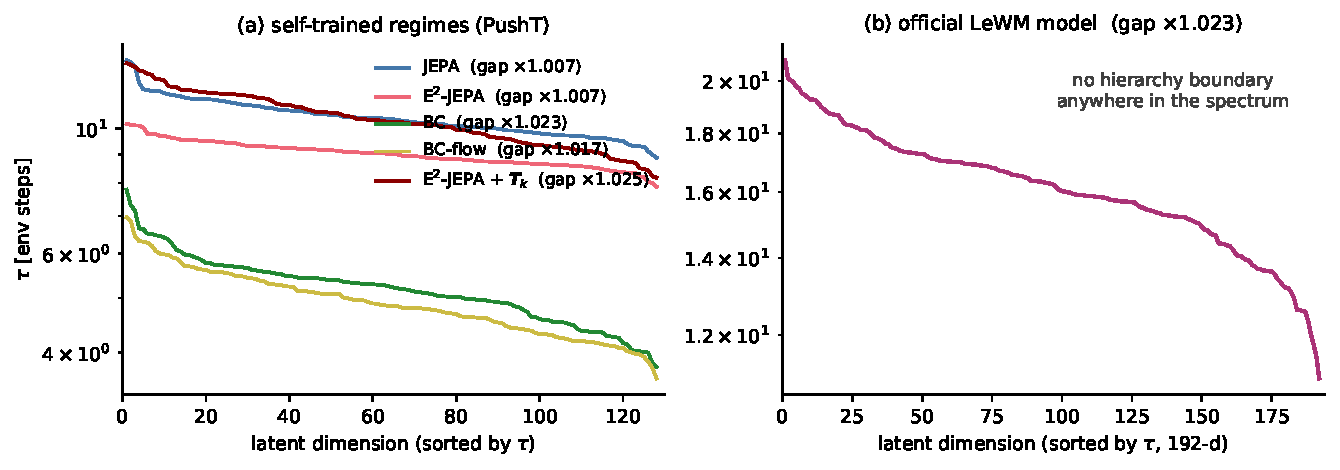
\includegraphics[width=\linewidth]{fig1.pdf}
    \caption{\textbf{Universal spectral gap collapse (measured).} (a)~Sorted $\tau$ spectra of five self-trained regimes on PushT---the four preliminary arms plus the temperature-vector arm tested in Section~4; each annotation gives the largest consecutive ratio. (b)~The official LeWM world model, measured on its own released training data under the identical protocol. No spectrum contains a boundary at which a hierarchy could be cut.}
    \label{fig:collapse}
\end{figure}

\subsection{The dynamics know the scales; the coordinates do not inherit them}

On the same E$^2$-JEPA latents, estimator A finds every dimension within $\tau = 9 \pm 1$ environment steps, while estimator B finds a spectrum spanning $0.1$--$20$ environment steps (Fig.~\ref{fig:ab}). The mismatch is the finding: the learned dynamics contain multi-scale structure, but the coordinate system does not express it. The external model sharpens this into a calibration result: LeWM's Jacobian spectrum contains exactly $7$ neutral modes ($|\lambda| \ge 1$ at every sampled context), matching the physical state dimension of PushT (agent position, block pose, velocities)---the model learned a unit-gain pass-through of the physical manifold---while its coordinate-level $\tau$ spectrum remains gapless. Structure exists in the dynamics; the objective never forces coordinates to inherit it.

\begin{figure}[t]
    \centering
    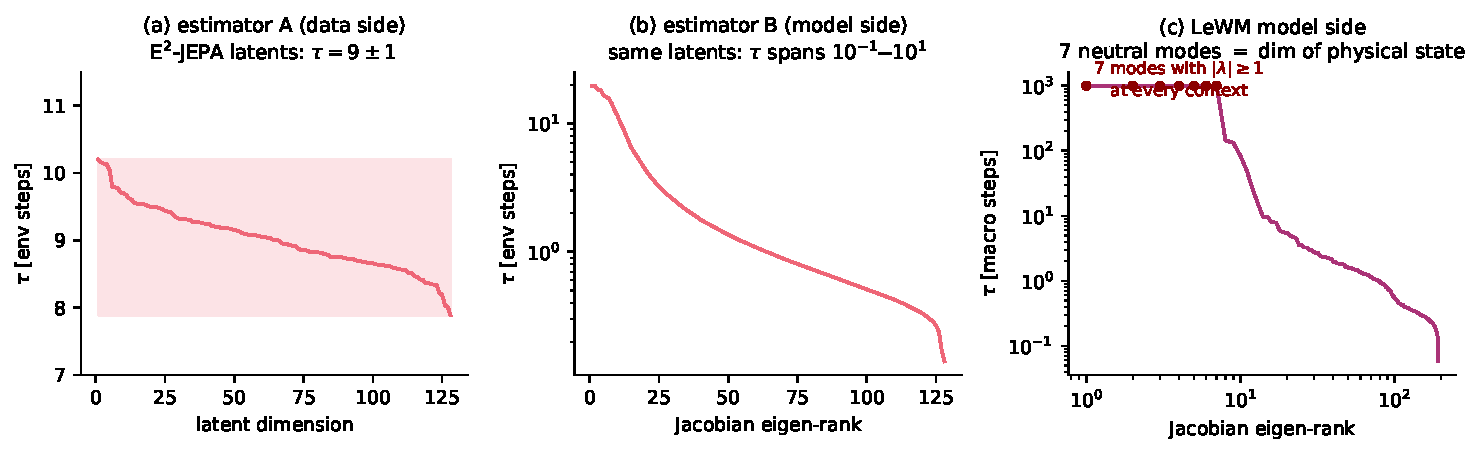
\includegraphics[width=\linewidth]{fig2.pdf}
    \caption{\textbf{A/B dissociation (measured).} (a)~Data-side $\tau$ of E$^2$-JEPA latents: one narrow band. (b)~Model-side $\tau$ of the same latents: three orders of magnitude. (c)~LeWM's model-side spectrum: exactly $7$ neutral modes, equal to the dimension of the physical state---the protocol recovers a known ground truth, and the dynamics provably contain the multi-scale structure that the coordinates lack.}
    \label{fig:ab}
\end{figure}

\subsection{Why scalar anti-collapse pressure cannot organize}

Existing regularizers prevent \emph{dimensional} collapse but are indifferent to temporal organization~\cite{vicreg2022,spectral2026}. Our measurements explain why this indifference is structural, through two complementary failure regimes (Fig.~\ref{fig:deadends}):

\begin{itemize}[leftmargin=1.5em]
    \item \textbf{Compressed representations have no room to organize.} LeWM's latent has participation ratio $6.2 \approx$ the physical state dimension: the data manifold is so low-dimensional that any half of any basis spans the entire state. Measured consequence: decoding block pose from the $\tau$-slow half vs.\ the $\tau$-fast half gives $R^2 = 0.61$ vs.\ $0.60$---flat, because a sufficient statistic cannot be split.
    \item \textbf{Overcomplete representations are homogenized.} Our E$^2$-JEPA latent has participation ratio $114$, leaving room for organization, but dense normalization mixes every dimension with every other, collapsing all data-side $\tau$ to $9 \pm 1$.
\end{itemize}

Either too little room or too much mixing---both regimes block spontaneous organization, so organization must be imposed by the objective function. This is the necessity argument for what follows.

\begin{figure}[t]
    \centering
    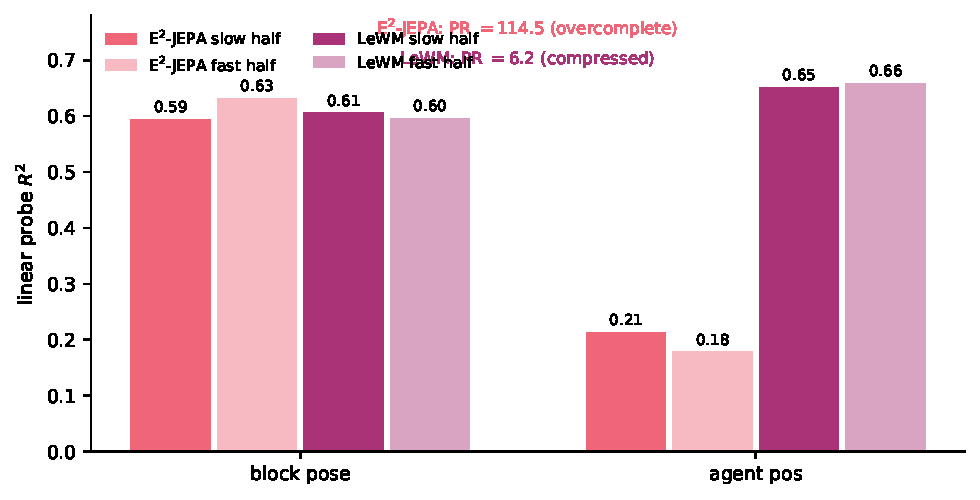
\includegraphics[width=0.8\linewidth]{fig3.pdf}
    \caption{\textbf{Two dead ends (measured).} Linear-probe $R^2$ for block pose and agent position, from the $\tau$-slow vs.\ $\tau$-fast half of each spectrum. LeWM (compressed, PR $= 6.2$) cannot be split because any half spans the whole physical state; E$^2$-JEPA (overcomplete, PR $= 114.5$) has room but the halves are interchangeable because per-dimension $\tau$ is homogenized. Information is present in both; temporal organization is present in neither.}
    \label{fig:deadends}
\end{figure}

\subsection{Entropy is an existence precondition for $\tau$}

Our energy-only control (free energy with the entropy term removed) collapses toward constant latents and measures \emph{pseudo-slow} $\tau$: median $15.6$, larger than any healthy model, while carrying near-zero information (probe $R^2 \le 0.42$, per-dimension std $0.003$; Fig.~\ref{fig:pseudo}). A constant signal has perfect autocorrelation and zero content. Hence $\tau$ is defined only where entropy is positive: the entropy term is not a regularization trick but the \emph{existence precondition of the metric this proposal is built on}. Any mechanism that manufactures a $\tau$ spectrum must therefore live inside a free-energy objective---which fixes the design space for the method.

\begin{figure}[t]
    \centering
    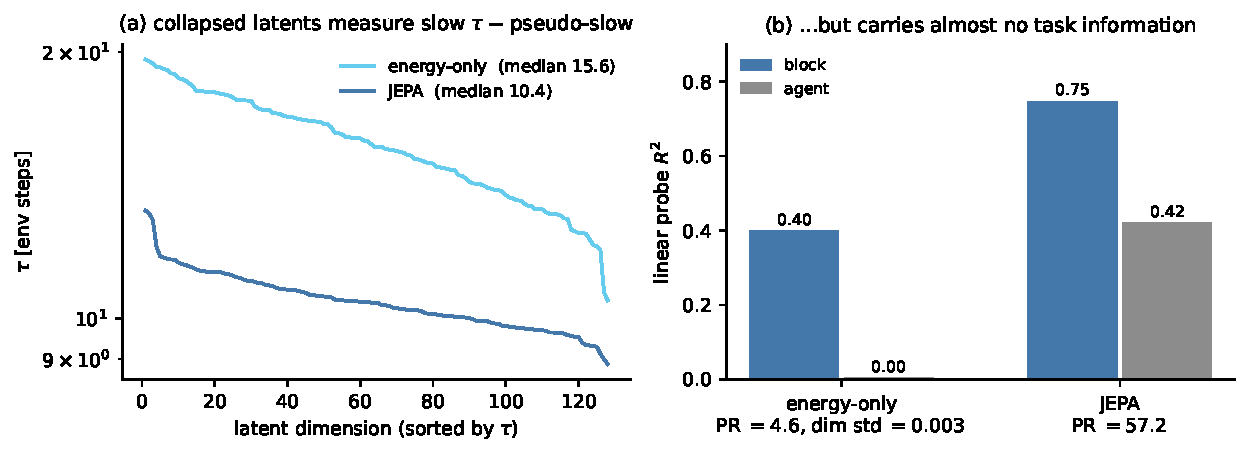
\includegraphics[width=\linewidth]{fig4.pdf}
    \caption{\textbf{Pseudo-slow $\tau$ (measured).} (a)~Removing the entropy term yields latents that measure \emph{slower} than any healthy model. (b)~Yet the same latents decode almost nothing, and their variance is degenerate. $\tau$ without entropy is meaningless, so the free-energy form is not an analogy but the existence precondition of the metric.}
    \label{fig:pseudo}
\end{figure}

\section{A First Mechanism, Tested: The Temperature Vector Is Insufficient}

The preliminary results constrain any fix: it must (i)~live inside a free-energy objective (Section~3.4), (ii)~act differentially across time scales, because a uniform scalar cannot (Section~3.3), and (iii)~exploit the structure already present in the dynamics (Section~3.2). The temperature vector is the natural first candidate under these constraints. A scalar $T$ applies one entropy pressure to all dimensions; because total entropy is identical for a temporally mixed and a temporally separated representation, the scalar objective cannot distinguish them---it is invariant under any relabeling of dimensions, so no gradient direction points from ``mixed'' toward ``organized.'' Replacing the scalar with a vector $\boldsymbol{T} = (T_1, \dots, T_K)$ over $K$ bands, each with its own per-dimension band entropy $S_k = \tfrac{1}{2|B_k|}\log\det\Sigma_k$,
\begin{equation}
    F = U - \sum_{k=1}^{K} T_k \, S_k ,
\end{equation}
breaks that permutation symmetry and creates a differential pressure under which, in principle, a mixed spectrum is no longer stationary. We trained this arm and scored it against criteria fixed before training.

\textbf{Preregistered test.} $K{=}4$ contiguous bands of 32 dimensions; a geometric temperature gradient $8{:}4{:}2{:}1$, normalized so the total entropy budget matches the scalar arm (only its distribution across bands differs); identical cooling schedule, data, batch, seed, and training protocol as the scalar E$^2$-JEPA arm. Criteria, fixed before the run: (1)~inter-band ratio of band-median $\tau \ge 1.5$ with monotonically decreasing medians; (2)~block-pose probe $R^2$ from the slow band exceeds the fast band by $\ge 0.2$; (3)~agent-position probe $R^2$ from the fast band $\ge 0.3$. A collapse guard requires every band's mean std $\ge 0.01$, so a degenerate solution cannot masquerade as success.

\begin{table}[t]
\centering
\begin{tabular}{lcc}
\hline
preregistered criterion & threshold & measured \\
\hline
inter-band ratio (monotone) & $\ge 1.5$ & $1.05\,/\,1.09\,/\,1.11$ \\
slow-band minus fast-band block probe & $\ge 0.2$ & $0.08$ \\
fast-band agent probe & $\ge 0.3$ & $0.10$ \\
\hline
\end{tabular}
\caption{The temperature-vector arm, scored against its preregistered criteria under the scalar arm's protocol. All three fail; the collapse guard passes (band stds $2.14$--$0.83$), so the negative is clean.}
\label{tab:tv}
\end{table}

\textbf{Result: all three criteria fail (Table~\ref{tab:tv}), and the failure is clean.} Every redistribution metric moved in the intended direction---band-median $\tau$ decreases monotonically $11.5 \to 9.2$, band std decreases $2.14 \to 0.83$, the block probe declines across bands $0.59 \to 0.46$, the $\tau$--block correlation strengthens to $+0.29$ (scalar arm: $+0.07$), and the participation ratio drops from $114.5$ to $45.7$, i.e.\ the representation is \emph{less} homogenized---yet the spectra of the two arms overlap almost exactly (Fig.~\ref{fig:mechanism}) and the fast variable is not retained anywhere.

\textbf{Diagnosis: temperature governs survival, not placement.} Entropy pressure decides whether information in a band survives the energy's incentive to drop it; it does not decide \emph{which band} content belongs to. The energy, meanwhile, prefers slow content everywhere (it is predictable) and removes fast content everywhere (it is not): it can only remove, never place. A band protected enough to retain fast content therefore also retains slow content---the two-dead-ends argument of Section~3.3 reproduces \emph{inside} the mechanism. The failure is thus not an implementation accident but the theory correctly predicting its own difficulty: organizing latents by time scale requires a force that \emph{places} information, and no member of the temperature family provides one.

\begin{figure}[t]
    \centering
    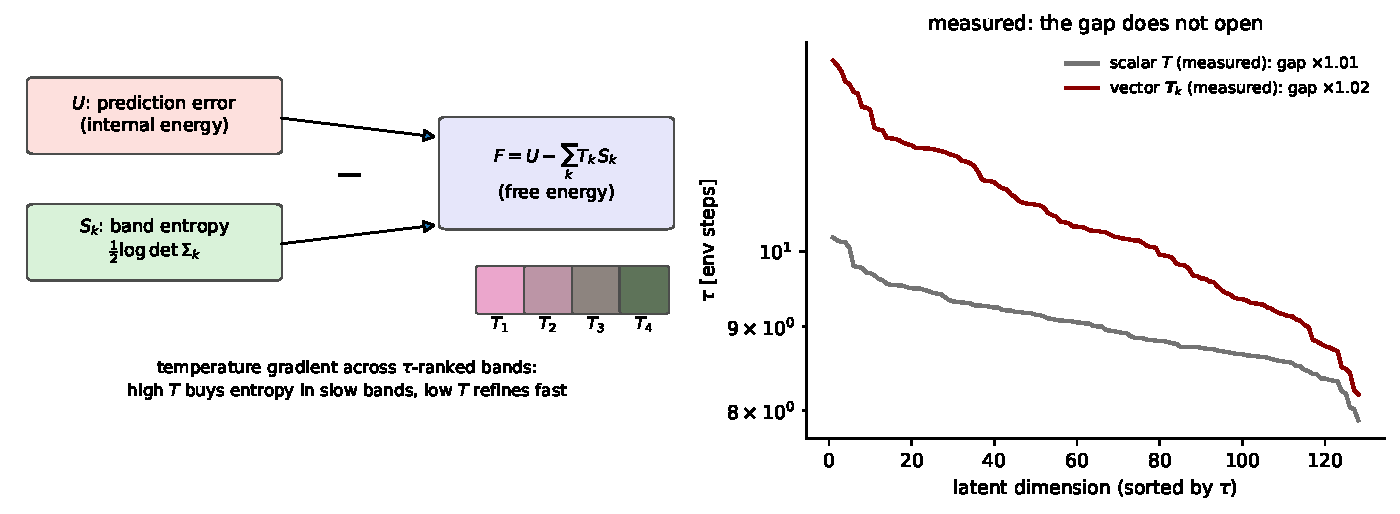
\includegraphics[width=\linewidth]{fig5.pdf}
    \caption{\textbf{Mechanism, tested.} Left: the free-energy mapping and the per-band temperature gradient that was trained. Right: the measured spectra of the scalar and vector arms---the vector moves every redistribution metric in the intended direction, but the spectra overlap; the gap does not open.}
    \label{fig:mechanism}
\end{figure}

\section{The Open Question, and How to Explore It}

The failure sharpens the problem: what force can \emph{place} information by time scale inside a trainable objective? This is the open core of temporal abstraction---if it were easy, hierarchical world models would not still treat their upper level's predictions as subgoals and fail~\cite{hilewm2026}. We structure the exploration as preregistered falsification loops around three falsifiable questions:

\begin{enumerate}[leftmargin=1.5em]
    \item \textbf{Open-loop or closed-loop fields.} The tested gradient was fixed a priori over fixed bands. Does coupling the temperature field to the measured spectrum---re-assigning bands by $\tau$ rank during training---escape the placement failure, or is every differential \emph{survival} pressure subject to it?
    \item \textbf{Coordinate side or dynamics side.} Fig.~\ref{fig:ab} shows the multiscale structure lives in the learned dynamics but is not inherited by the coordinates. Is enforcement more natural where the structure already is---on the eigen-structure of the one-step Jacobian---than on the coordinates it fails to reach?
    \item \textbf{Objective or architecture.} If no objective-side force suffices, temporal organization is an architectural constraint, as hierarchy-by-design lines assume implicitly. The $\tau$ protocol can decide this empirically instead of by taste.
\end{enumerate}

Each loop is a single-arm training plus one $\tau$ measurement, every acceptance criterion is fixed before the run, and the referee is the same protocol that audited the external model. When any mechanism passes, the plan converges on the endgame: hierarchy boundaries cut at the measured gap, and subgoals admitted only where their $\tau$ matches the lower level's reachable horizon, backtested on the failing interface of~\cite{hilewm2026} ($38.7\%$ vs.\ $73.3\%$)---the direct test of whether the metric repairs the interface it was motivated by. Transfer to a different embodiment is optional scope, not a claim.

\section{Risk Assessment}

The proposal has already absorbed its first preregistered falsification: the temperature vector failed, was diagnosed, and narrowed the hypothesis space---survival is not placement. The same discipline governs the remaining risk, that no objective-side force organizes latents at all. That terminal negative would itself be a result: it would locate temporal organization on the architectural side of the design space, and it would be published together with the protocol that proved it. The measurement contribution---the $\tau$ referee, the universality of spectral gap collapse, and the two-dead-ends diagnosis---stands independently of which way the exploration resolves.

\section{Conclusion}

Self-organized latents never separate time scales---five training regimes and an independent deployed model agree, and the temperature-vector arm joins them (Fig.~\ref{fig:mechanism}). The first-principles fix suggested by the measurements redistributes variance but not content: temperature preserves information, and only placement can organize it. What force can place information by time scale inside a trainable objective is genuinely open; this proposal brings to it a referee that measures, criteria fixed in advance, and an endgame that matters for hierarchical planning.

\bibliographystyle{plain}
\bibliography{refs}

\end{document}
